% Authors: Taejin Hwang, Justin Yu
% Emails: taejin@berkeley.edu, justinvyu@berkeley.edu

% Note: This specific reboot is specific to Sahai's Fall 2019 iteration of 16B. It was created by merging the bode_plots_intro and bode_filters question. For future semesters, it'll probably be more appropriate to use the two together.

\qns{Bode Plots for Filters}
\pgfplotsset{compat=1.9, every tick label/.append style={font=\normalsize}} 

\meta{Prereqs: Transfer Functions, Complex magnitude and phases, plotting functions}

Bode plots provide us with a simple and easy tool to plot these transfer functions by hand. \textbf{Always remember that Bode plots are an approximation}; if you want the precisely correct plots, you need to use numerical methods (like solving using MATLAB or IPython).

When we make Bode plots, we plot the frequency and magintude on a logarithmic scale and the angle in either degrees or radians. 
We use the log scale because it allows us to break up complex transfer functions into its constituent components. 

% We note that every transfer function can be written in its \textit{rational transfer function form,} which is a product of poles and zeros. When making the Bode plot (and plotting using a logarithmic unit), we treat each individual pole and zero independently, and then add them back together at the end. This question will examine the Bode plots of single zeros and poles, and we can generalize these plots to create a Bode plot for any transfer function.

When plotting the transfer function, the most important quantity to look at is its cutoff frequency $\omega_{c}.$ 
We will take a look the individual Bode plots for low and high pass filters, and then look at how the Bode plot for a bandpass filter is constructed. 

\meta{
  Note: This semester, drawing straight-line approximations to Bode plots are no longer in scope.
  However, we will motivate the process of drawing straight line approximations by looking at points for which $\omega \approx 0, \omega = \omega_c,$ and $\omega >> \omega_c.$
}

\begin{enumerate}

\qitem Let's start by taking a look at $H(j \omega) = X(j \omega)Y(j \omega)$, the product of two transfer functions $X$ and $Y$.
\begin{enumerate}
    \qitem How can you graph $|H(j \omega)|$ using the graphs of $|X(j \omega)|$, $|Y(j \omega)|$?
    \qitem How does this compare when graphing $\log |H(j \omega)|$ using the graphs of $\log |X(j \omega)|$, $\log |Y(j \omega)|$?
    \qitem What is the relationship between $\angle H(j \omega), \angle X(j \omega),$ and $\angle Y(j \omega)?$
\end{enumerate}

\sol{
\begin{enumerate}
  \qitem To get $H(j \omega),$ we would have to multiply the graphs of $|X(j \omega)|$ and $|Y(j \omega)|.$
  \qitem Since $\log |H(j \omega)| = \log |X(j \omega)| + \log |Y(j \omega)|,$ we would have to add the graphs of $\log X(j \omega)$ and $\log Y(j \omega)$ which is much easier to do.
  \qitem $H(j \omega) = |H(j \omega)| e^{j \angle H(j \omega)} = |X(j \omega)| e^{j \angle X(j \omega)} \cdot |Y(j \omega)| e^{j \angle Y(j \omega)} = 
  |X(j \omega)| |Y(j \omega)| e^{(\angle X(j \omega) + \angle Y(j \omega))}.$ \\
  Therefore, $\angle H(j \omega) = \angle X(j \omega) + \angle Y(j \omega).$
\end{enumerate}
}

\qitem Let $H(j \omega) = \frac{1}{1 + j \frac{\omega}{\omega_c}}$. This transfer function models the effect of a low pass filter, and has cutoff frequency $\omega_{c}.$

\begin{enumerate}
    \qitem Find $|H(j \omega)|$ and $\angle H(j \omega)$.

    \sol { 
      $|H(j \omega)| = \frac{1}{\sqrt{1 + (\frac{\omega}{\omega_{c}})^2}}.$ and $\angle H(j \omega) = - \tan^{-1} (\frac{\omega}{\omega_c})$
    }

    \qitem Again, \textbf{fill in the following table to analyze the magnitude and phase at the three regions $\omega << \omega_{c}$, $\omega = \omega_{c}$, and $\omega >> \omega_{c}$.}

    \ws{
      \begin{table}[ht!]
        \centering
        \begin{tabular}{| l | >{\centering\arraybackslash}m{6em} | >{\centering\arraybackslash}m{6em} | >{\centering\arraybackslash}m{6em} |} 
        \cline{2-4}
        \multicolumn{1}{l|}{}& $\omega << \omega_{c}$ & $\omega = \omega_{c}$ & $\omega >> \omega_{c}$ \\
        \hline
        &&&\\
        $H(j \omega)$        &                      &                     &                      \\
        &&&\\
        \hline
        &&&\\
        $|H(j \omega)|$      &                      &                     &                      \\
        &&&\\
        \hline
        &&&\\
        $\angle H(j \omega)$ &                      &                     &                      \\
        &&&\\
        \hline
        \end{tabular}
      \end{table}
    }

    \sol{
      \begin{table}[ht!]
        \centering
        \begin{tabular}{| l | >{\centering\arraybackslash}m{6em} | >{\centering\arraybackslash}m{6em} | >{\centering\arraybackslash}m{6em} |} 
        \cline{2-4}
        \multicolumn{1}{l|}{}& $\omega << \omega_{c}$ & $\omega = \omega_{c}$ & $\omega >> \omega_{c}$ \\
        \hline
        &&&\\
        $H_z(\omega)$        &   1                 &       $\frac{1}{1 + j}$             &         $\frac{\omega_{c}}{\omega}$           \\
        &&&\\
        \hline
        &&&\\
        $|H_z(\omega)|$      &   1                   &      $\frac{1}{\sqrt{2}}$              &      $\frac{\omega_{c}}{\omega}$              \\
        &&&\\
        \hline
        &&&\\
        $\angle H_z(\omega)$ &   0                   &      $-\frac{\pi}{4}$               &    $-\frac{\pi}{2}$                    \\
        &&&\\
        \hline
        \end{tabular}
      \end{table}
    }

    \qitem \textbf{Draw a sketch of $|H(j \omega)|$ and $\angle H(j \omega)$ using the points, filled in the chart above.}

    \sol{
      \begin{figure}[!ht]
        \centering
        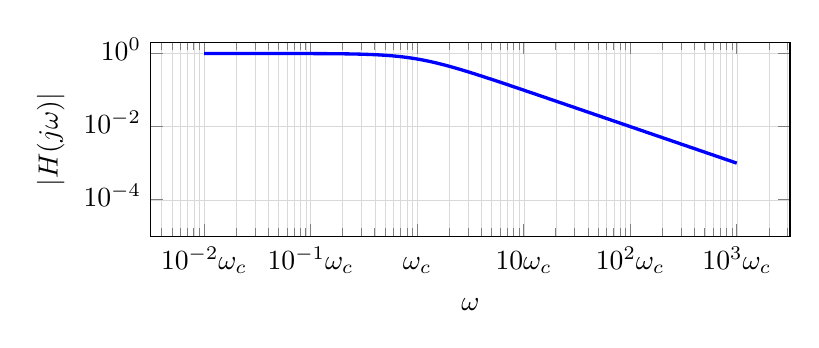
\begin{tikzpicture}[
            declare function={
              mag(\omega)= 1 / sqrt(1 + (\omega / 10^2)^2)
              % Bode approximation
              % (\omega < 10^2) * (1) +
              %           (\omega >= 10^2) * (10^2 / \omega)
             ;
            }
        ]
        \begin{loglogaxis}[
          typeset ticklabels with strut,
          ymin=0.00001, ymax=2, ylabel=$|H(j \omega)|$,
          xticklabels = {$10^{-3} \omega_{c}$, $10^{-2} \omega_{c}$, $10^{-1} \omega_{c}$,
          $\omega_{c}$, $10 \omega_{c}$, $10^{2} \omega_{c}$, $10^{3} \omega_{c}$}, xlabel=$\omega$,
          , 
          domain=10^0:10^5, 
          grid=both, grid style={line width=.1pt, draw=gray!30},
          width=\textwidth * 0.8,
          height=\textwidth / 3,
          samples = 500
        ]
        \addplot [blue,very thick] {mag(x)};
        \end{loglogaxis}
        \end{tikzpicture}
      \end{figure}

      \begin{figure}[!ht]
        \centering
        \hspace{0.7 cm}
        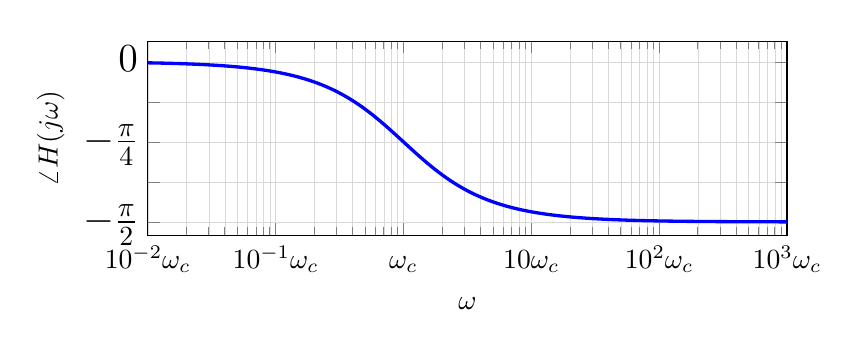
\begin{tikzpicture}[
            declare function={
              mag(\omega)= -rad(atan(\omega / 10^2))
              % Bode approximation
              % (\omega < 10^2) * (0) + and(\omega >= 10^2, \omega < 10^4) * (pi / 4 * (-log10(\omega) + 2))
              %           + (\omega >= 10^4) * (-pi / 2)
             ;
            }
        ]
        \begin{semilogxaxis}[
          typeset ticklabels with strut,
          ymin=-1.7, ymax=0.2, ylabel=$\angle H(j \omega)$, ytick={0, -pi/8, -pi/4, -3 * pi/8, -pi/2}, 
          yticklabels={$0$, $\,$, $-\frac{\pi}{4}$, $\,$, $-\frac{\pi}{2}$},
          yticklabel style={font=\Large},
          xmin=10^0, xmax=10^5, xlabel=$\omega$,
          xticklabels = {$10^{-2} \omega_{c}$, $10^{-1} \omega_{c}$, $\omega_{c}$,
          $10 \omega_{c}$, $10^{2} \omega_{c}$, $10^{3} \omega_{c}$}, 
          domain=10^0:10^5, 
          grid=both, grid style={line width=.1pt, draw=gray!30},
          width=\textwidth * 0.8,
          height=\textwidth / 3,
          samples = 500
        ]
        \addplot [blue,very thick] {mag(x)};
        \end{semilogxaxis}
        \end{tikzpicture}
      \end{figure}
    }

\end{enumerate}

\ws{
  \begin{figure}[!ht]
    \centering
    \begin{minipage}[b]{0.37\textwidth}
    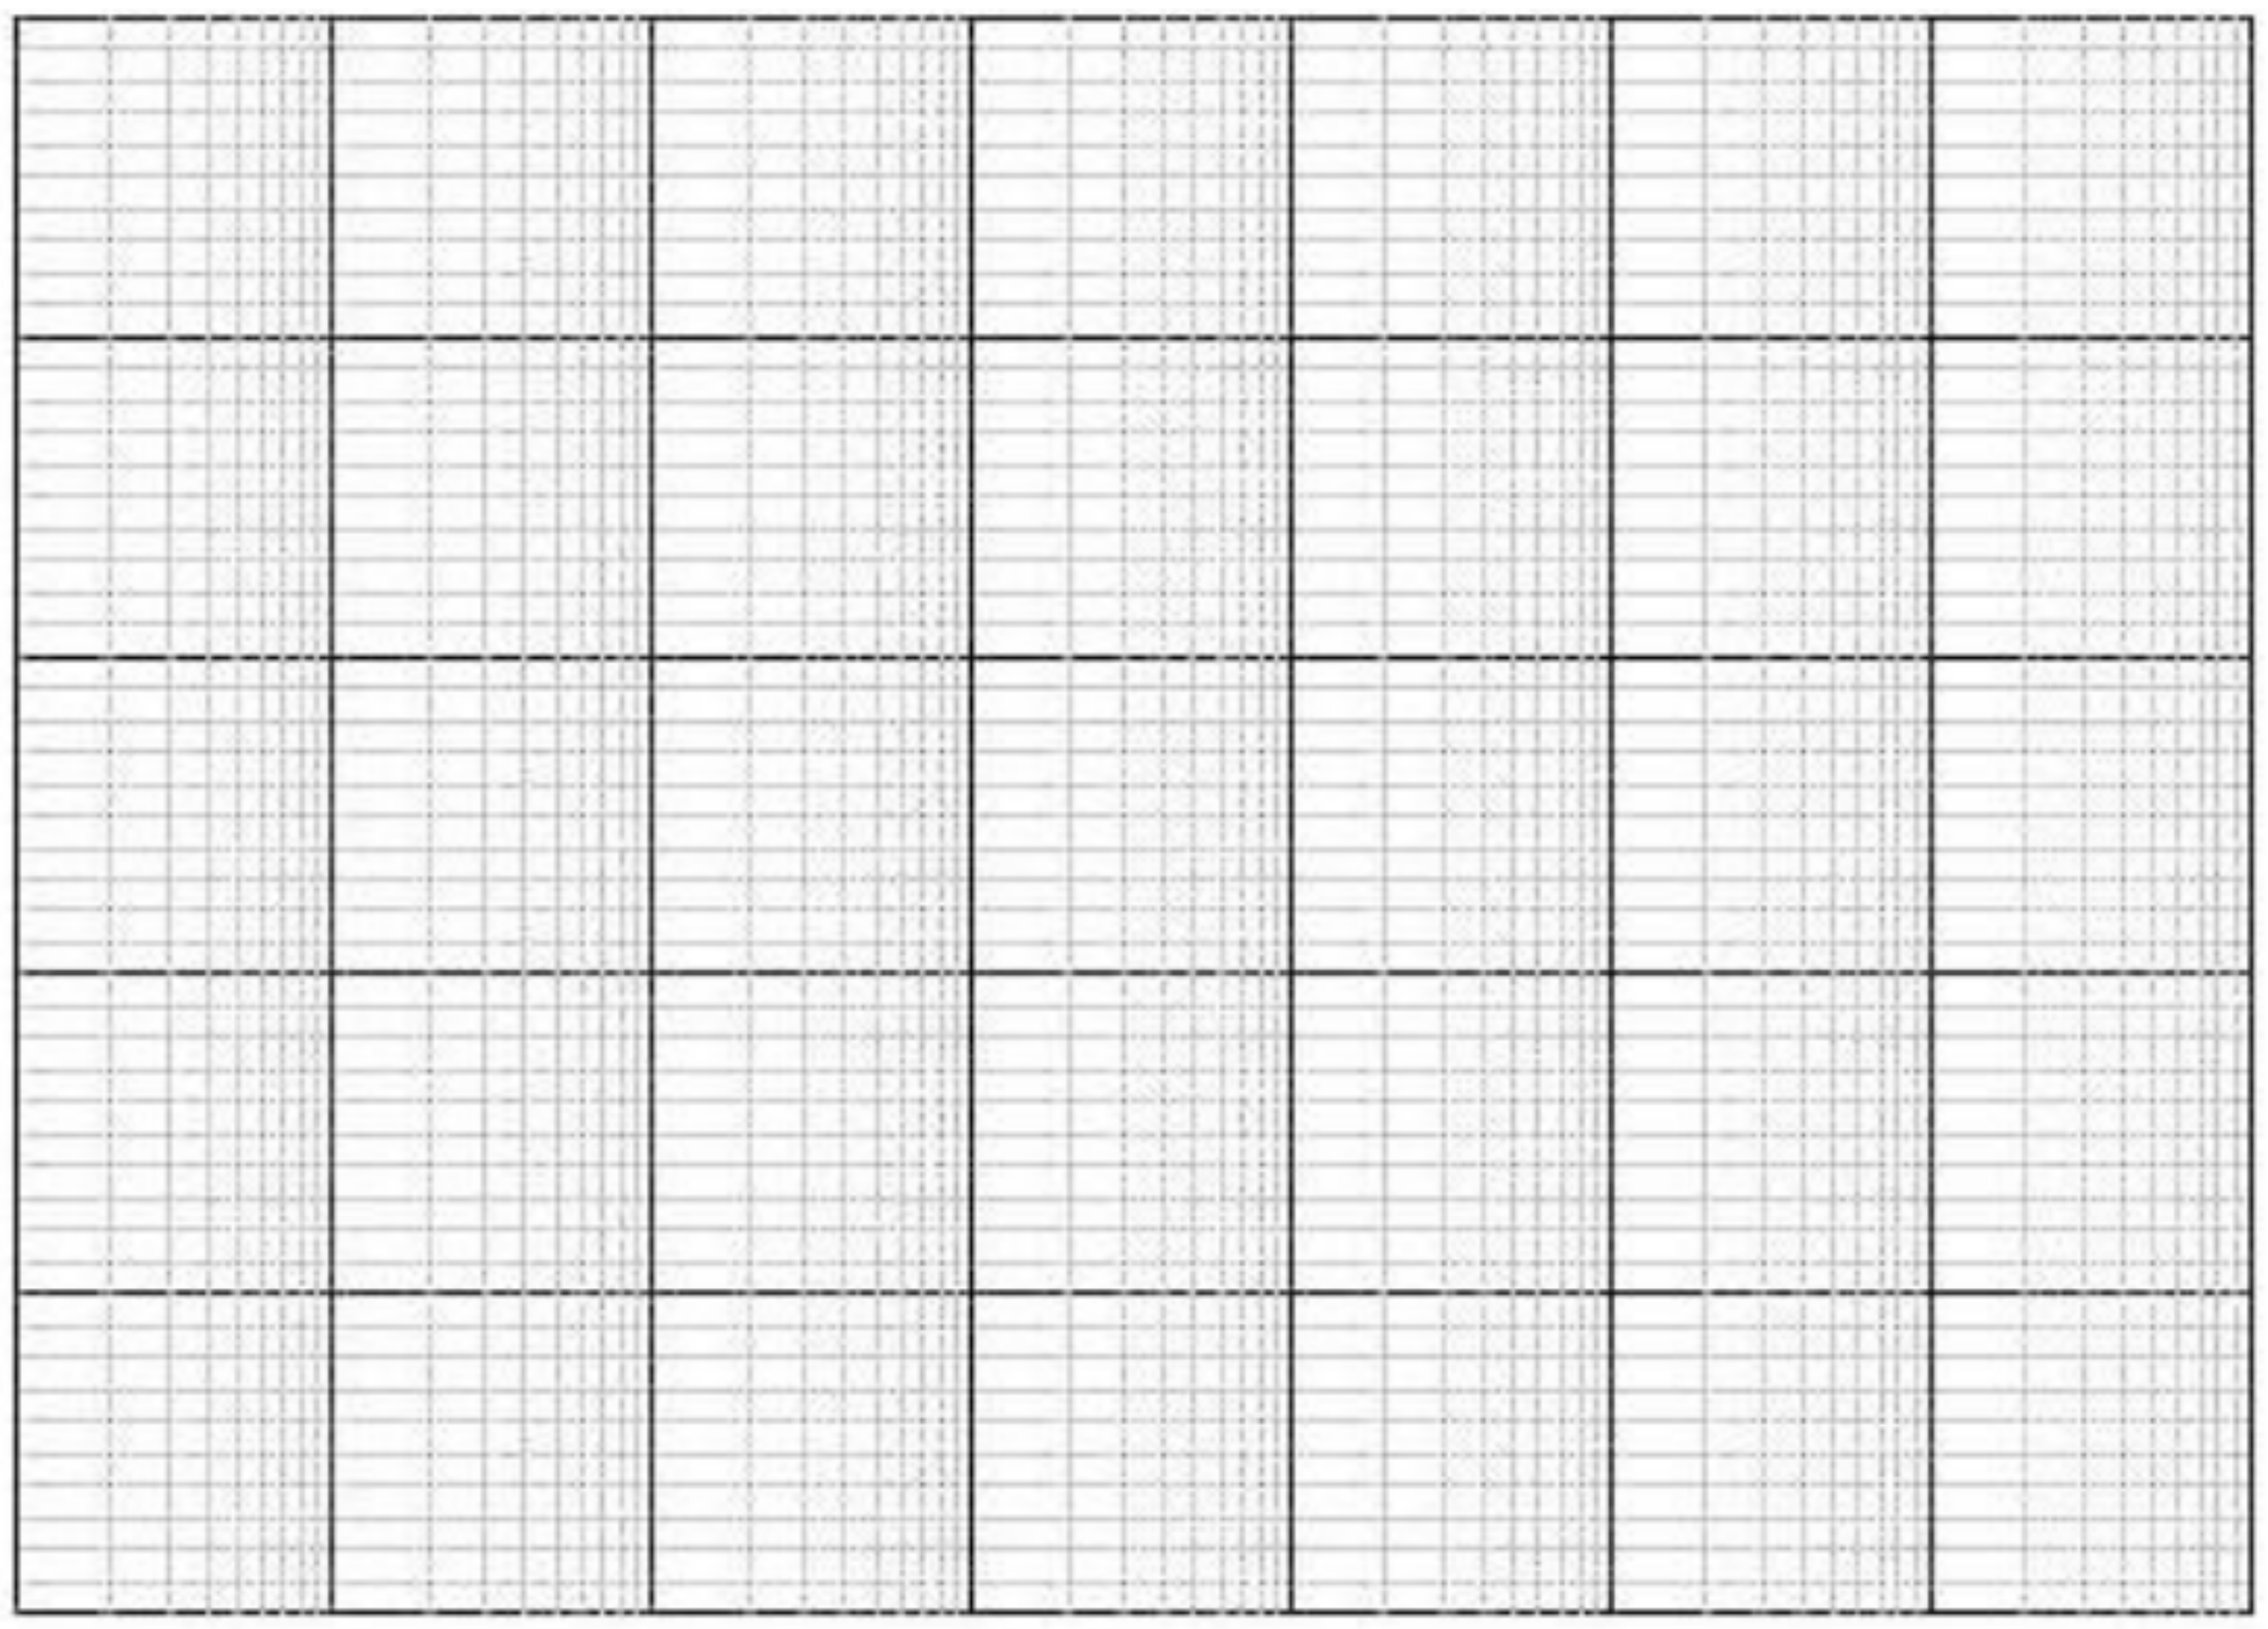
\includegraphics[width=1.0\textwidth]{\bank/transfer/figures/bodeblank}
      \caption*{$|H(j \omega)|$}
    \end{minipage}
    \hspace{2cm}
    \begin{minipage}[b]{0.37\textwidth}
    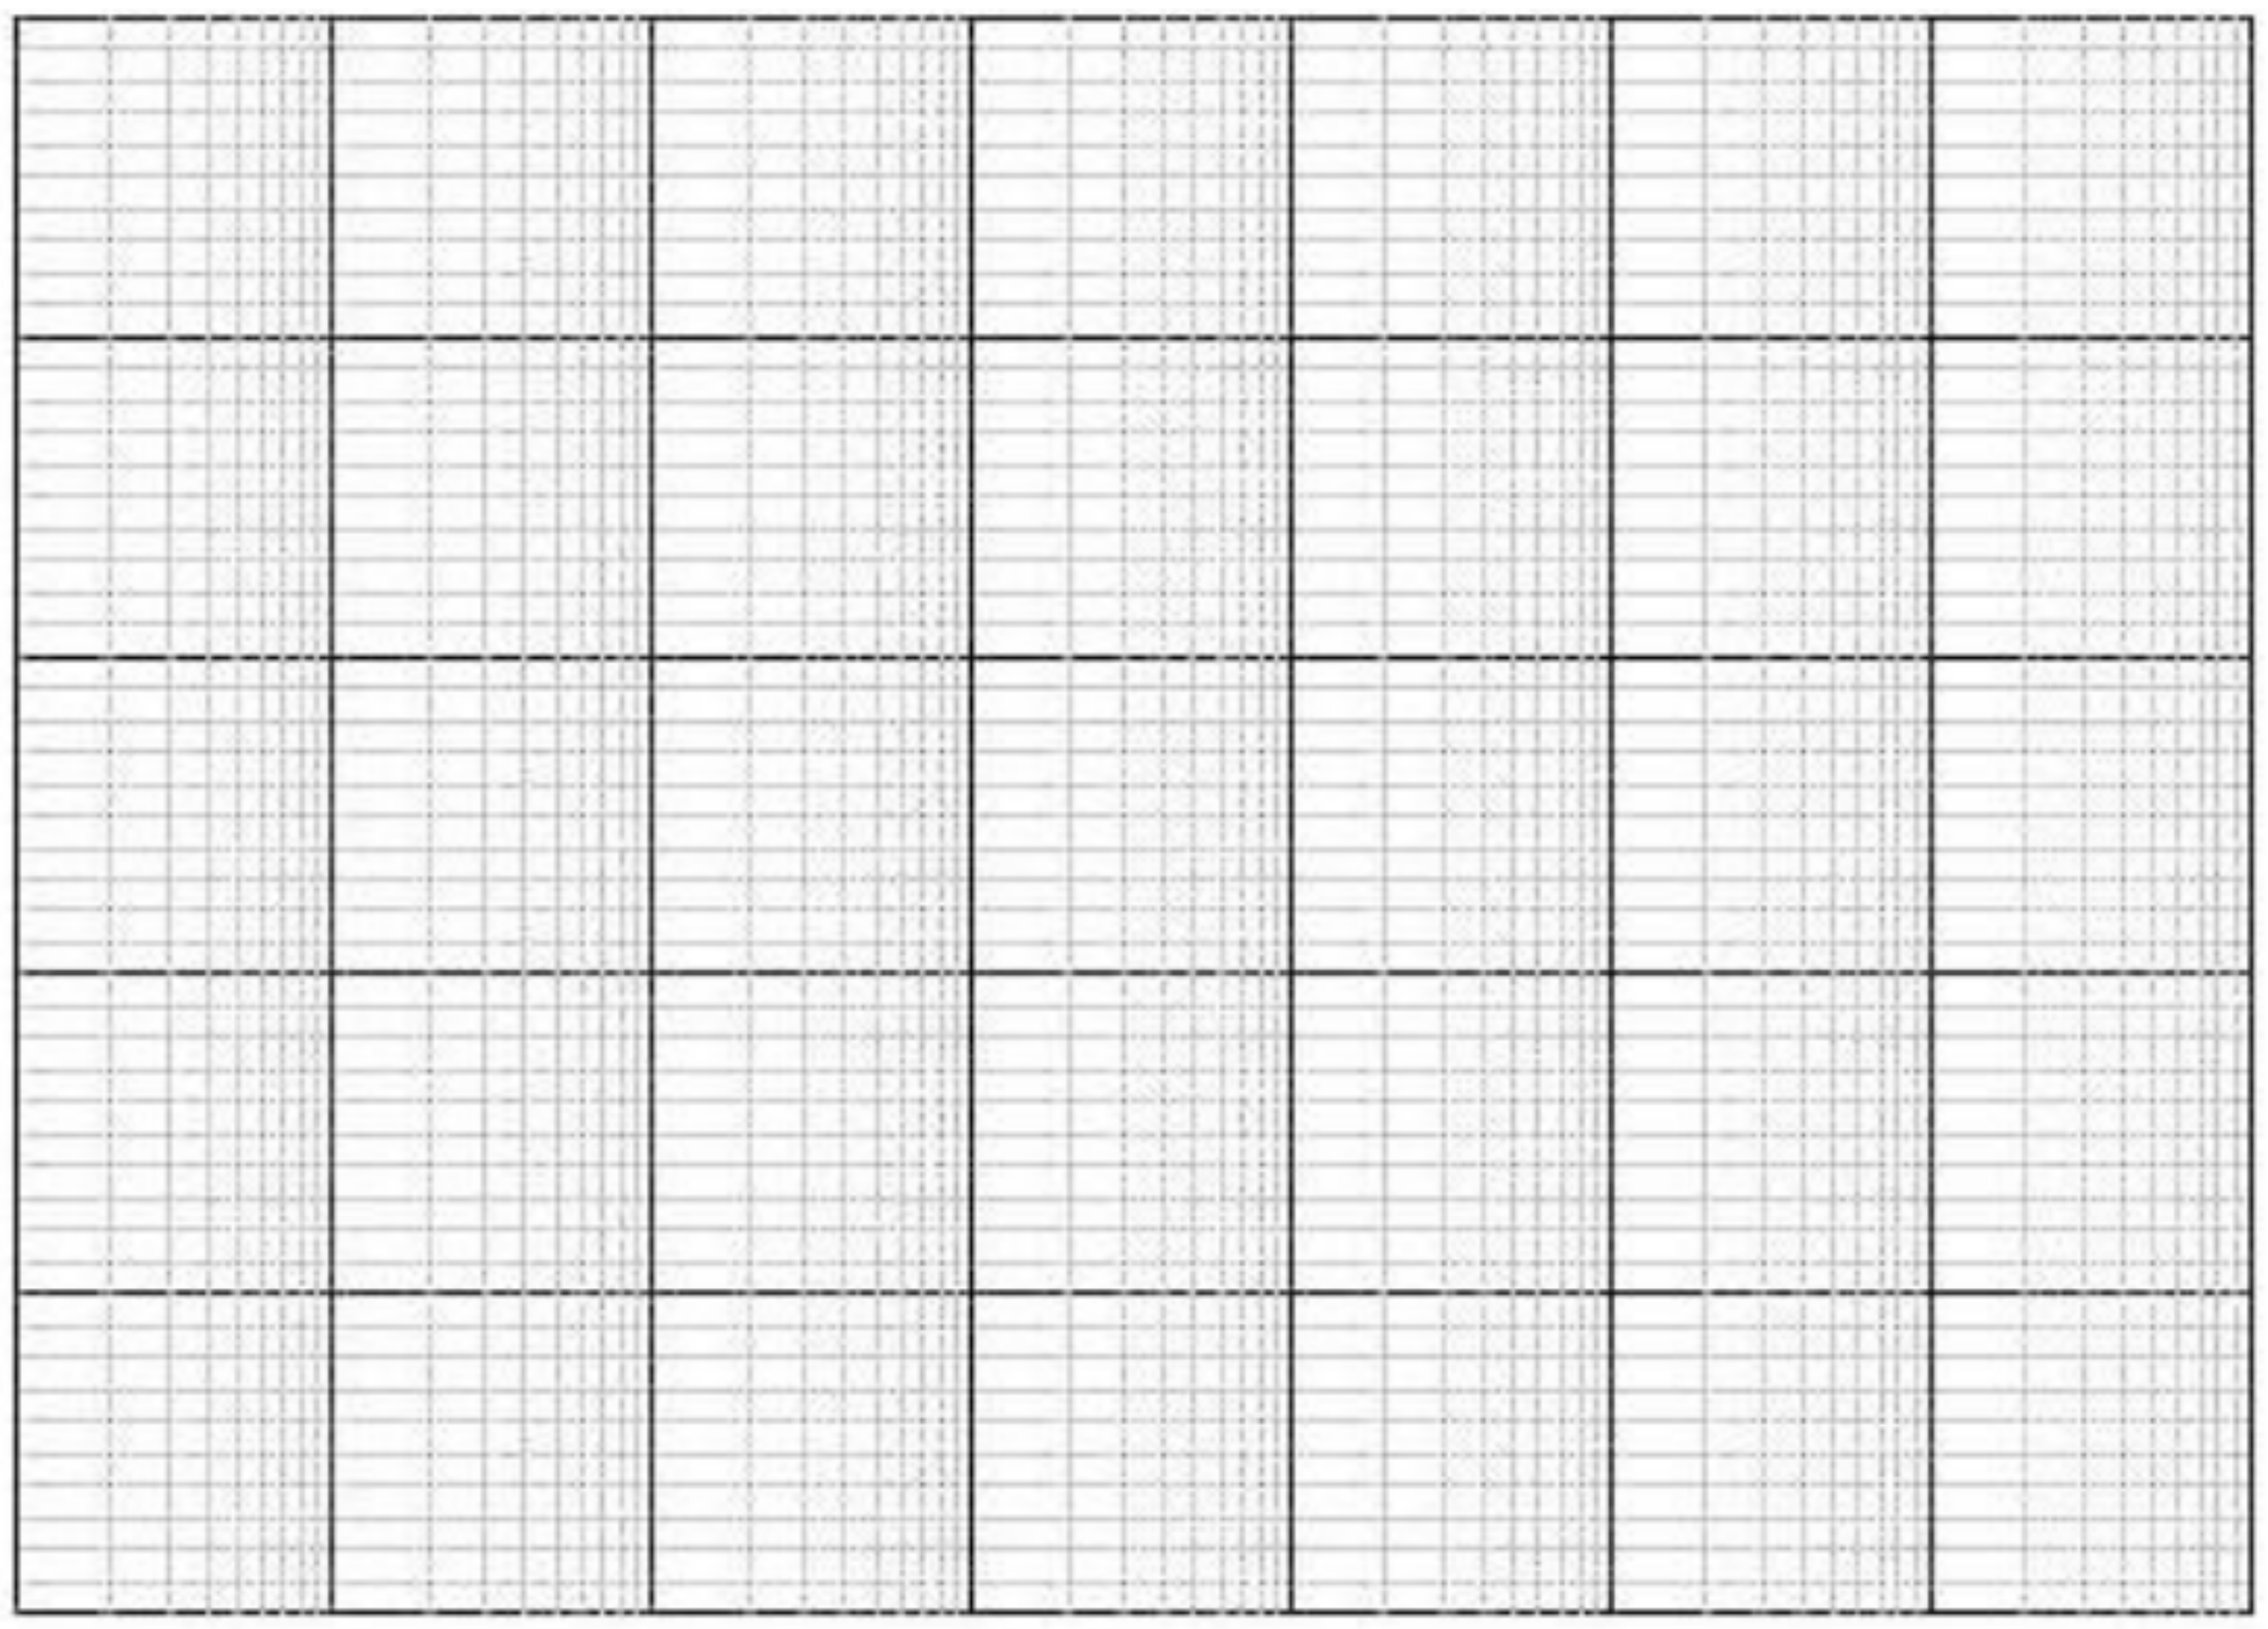
\includegraphics[width=1.0\textwidth]{\bank/transfer/figures/bodeblank}
      \caption*{$\angle H(j \omega)$}
    \end{minipage}
  \end{figure}
}

\qitem Let $H(j \omega) = j\omega$. This transfer function does not have a cutoff frequency, but its behavior will prove to be useful when looking at a high-pass filter.
\begin{enumerate}
  \qitem \textbf{Find $|H(j \omega)|$ and $\angle H(j \omega)$}.
  \qitem \textbf{Sketch them down below.}

\ws{
  \begin{figure}[!ht]
    \centering
    \begin{minipage}[b]{0.37\textwidth}
    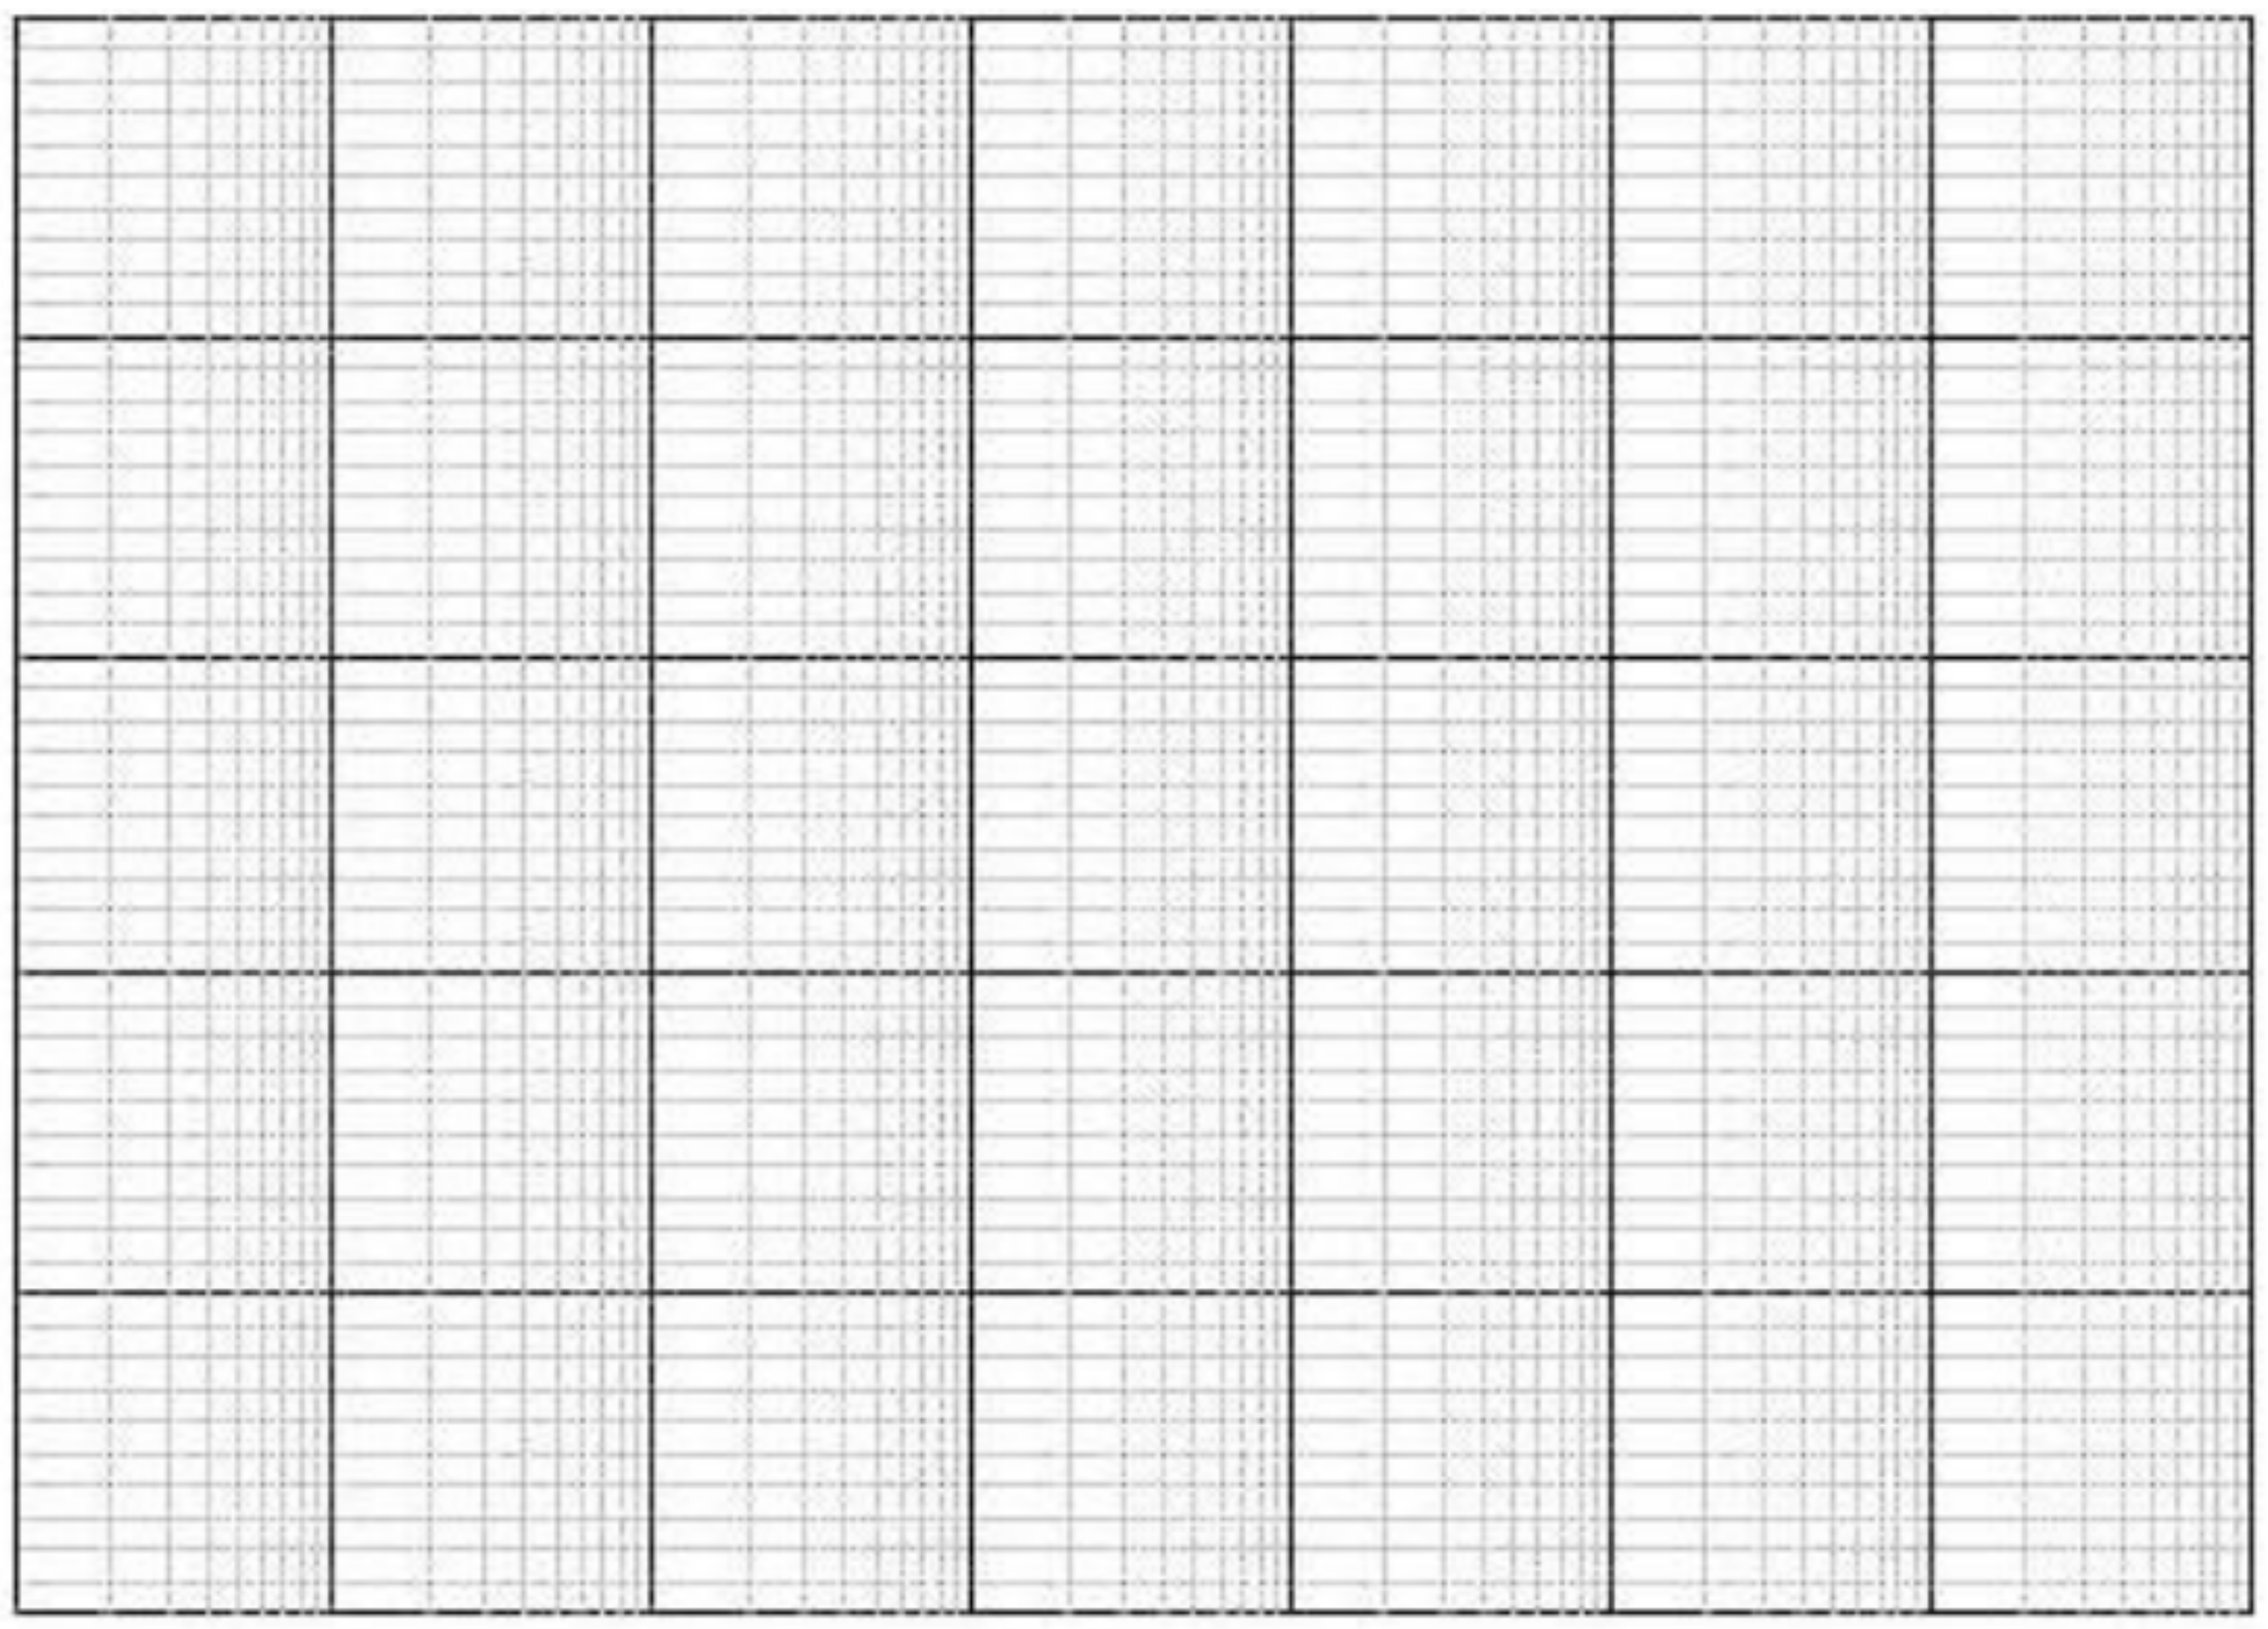
\includegraphics[width=1.0\textwidth]{\bank/transfer/figures/bodeblank}
      \caption*{$|H(j \omega)|$}
    \end{minipage}
    \hspace{2 cm}
    \begin{minipage}[b]{0.37\textwidth}
    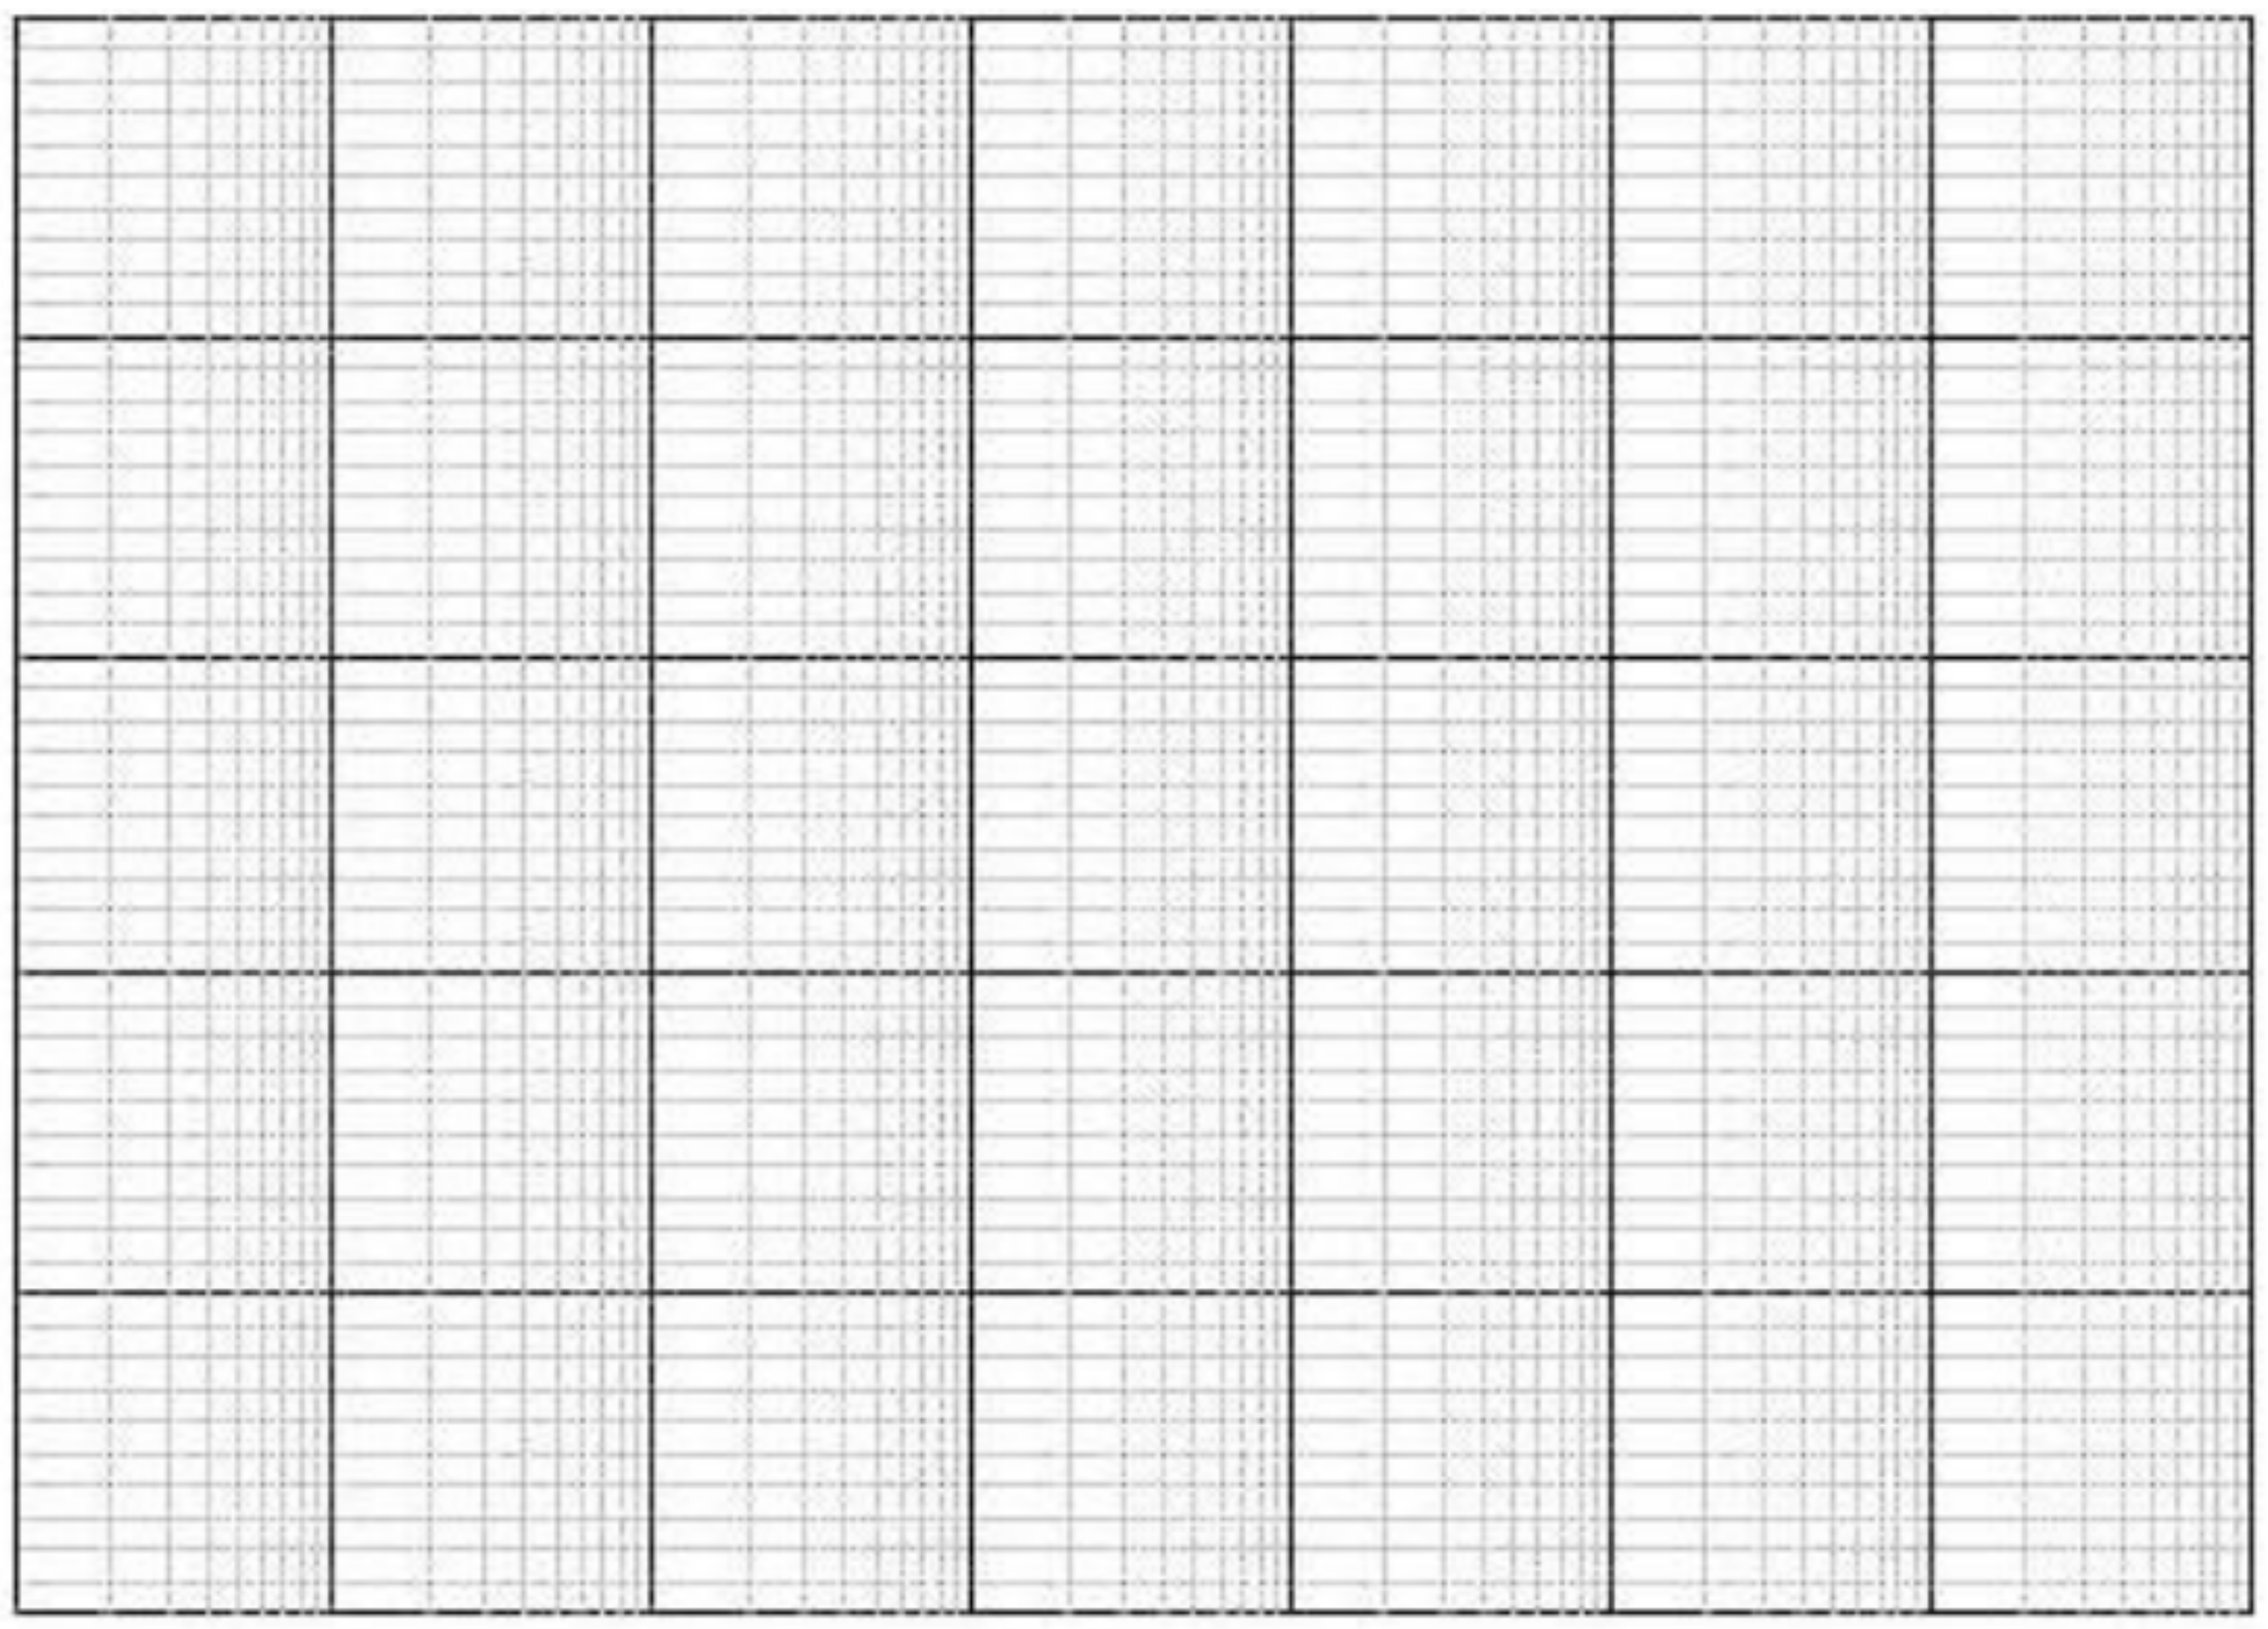
\includegraphics[width=1.0\textwidth]{\bank/transfer/figures/bodeblank}
      \caption*{$\angle H(j \omega)$}
    \end{minipage}
  \end{figure}
}

\end{enumerate}

\sol{
\begin{enumerate}
  \item $|H(j \omega)| = {\omega},$ and $\angle H(j \omega) = \frac{\pi}{2}.$
  \item $\,$
\begin{figure}[!ht]
  \centering
  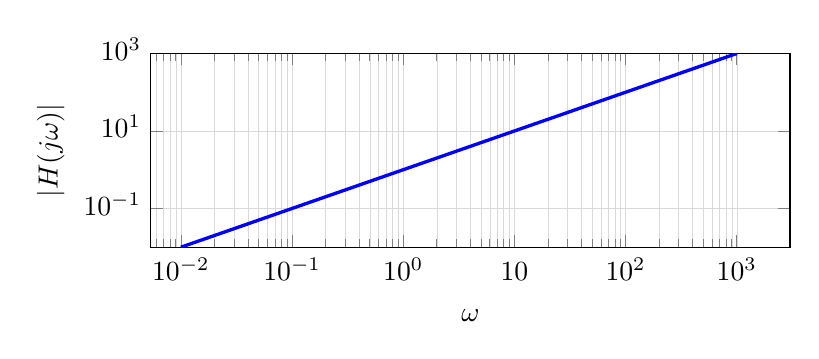
\begin{tikzpicture}[
      declare function={
        mag(\omega)= \omega
       ;
      }
  ]
  \begin{loglogaxis}[
    typeset ticklabels with strut,
    ymin=0.01, ymax=1000, ylabel=$|H(j \omega)|$,
    xticklabels = {$10^{-3}$, $10^{-2}$, $10^{-1}$,
    $10^{0}$, $10$, $10^{2}$, $10^{3}$}, xlabel=$\omega$,
    , 
    domain=10^-2:10^3, 
    grid=both, grid style={line width=.1pt, draw=gray!30},
    width=\textwidth * 0.8,
    height=\textwidth / 3
  ]
  \addplot [blue,very thick] {mag(x)};
  \end{loglogaxis}
  \end{tikzpicture}

  \vspace{0.3 cm}
\end{figure}

\newpage

\begin{figure}[!h]
  \centering
  \hspace{0.9 cm}
  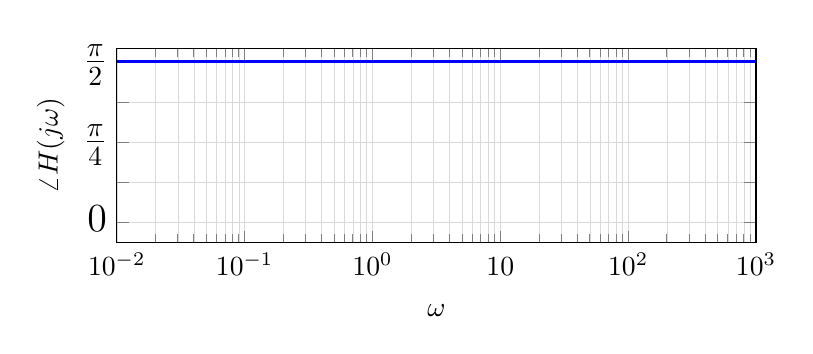
\begin{tikzpicture}[
      declare function={
        phase(\omega)= pi / 2
       ;
      }
  ]

  \begin{semilogxaxis}[
    typeset ticklabels with strut,
    ymin=-0.2, ymax=1.7, ylabel=$\angle H(j \omega)$, ytick={0, pi/8, pi/4, 3 * pi/8, pi/2}, 
    yticklabels={$0$, $\,$, $\frac{\pi}{4}$, $\,$, $\frac{\pi}{2}$},
    yticklabel style={font=\Large},
    xmin=10^-2, xmax=10^3, xlabel=$\omega$,
    xticklabels = {$10^{-3}$, $10^{-2}$, $10^{-1}$,
    $10^{0}$, $10$, $10^{2}$, $10^{3}$}, 
    domain=10^-2:10^3, 
    grid=both, grid style={line width=.1pt, draw=gray!30},
    width=\textwidth * 0.8,
    height=\textwidth / 3
  ]
  \addplot [blue,very thick] {phase(x)};
  \end{semilogxaxis}
  \end{tikzpicture}
\end{figure}

\end{enumerate}
}

\qitem Now let's go back to the low-pass filter with transfer function 
\begin{equation}
H(j \omega) = \frac{1}{j\omega R_{1}C_{1} + 1} 
\end{equation}

Let $R_{1} = 100 \Omega$ and $C_{1} = 100 pF$
\begin{enumerate}
  \qitem What is the cutoff frequency of this filter?

  \sol{
  $\omega_{c} = \frac{1}{R_{1}C_{1}} = \frac{1}{10^{2} \cdot 10^{-10}} = 10^{8}$
  }
  \qitem Sketch its phase and magnitude.

  \sol{
  Magnitude (log-log scale): The magnitude of $H(j \omega)$ is close to 1 until $\omega_{c}$, after which it starts decreasing at a quick rate.

  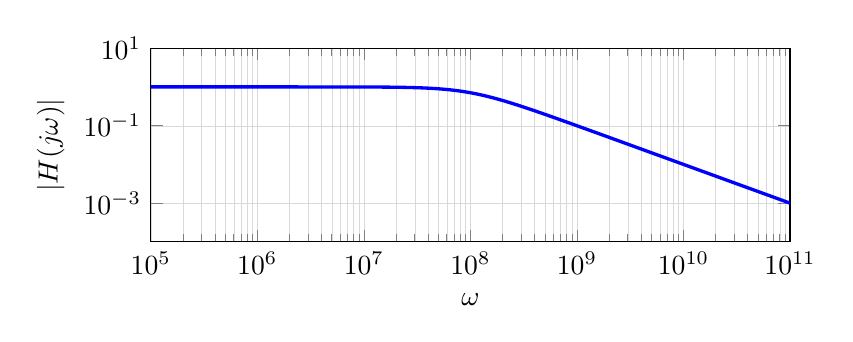
\begin{tikzpicture}[
    declare function={
      mag(\omega)= 1 / sqrt(1 + (\omega / 10^8)^2)
      % Bode approximation
      % (\omega < 10^8) * (1) +
      %           (\omega >= 10^8) * (10^8 / \omega)
     ;
    }
  ]
    \begin{loglogaxis}[
      ymin=0.0001, ymax=10, ylabel=$|H(j \omega)|$,
      xmin=10^5, xmax=10^11, xlabel=$\omega$,
      domain=10^5:10^11,
      grid=both, grid style={line width=.1pt, draw=gray!30},
      width=\textwidth * 0.8,
      height=\textwidth / 3,
      samples=500
    ]
      \addplot [blue,very thick] {mag(x)};
    \end{loglogaxis}
  \end{tikzpicture}
  
  Phase (semi-log scale): The phase of $H(j \omega)$ can be approximated using the three points from the previous parts. When $\omega \approx 0, \angle H(j \omega) \approx 0,$ when $\omega = \omega_{c}, \angle H(j \omega) = \frac{\pi}{4},$ and when $\omega >> \omega_{c}, \angle H(j \omega) = \frac{\pi}{2}.$

  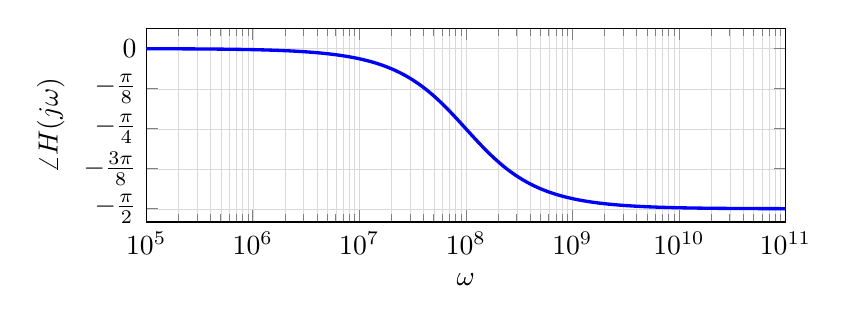
\begin{tikzpicture}[
    declare function={
      phase(\omega)= -rad(atan(\omega / 10^8))
      % Bode approximation
      % phase(\omega)= (\omega < 10^7) * (0) +
      %           and(\omega >= 10^7, \omega < 10^9) * (-pi / 4 * (log10(\omega) - 7)) +
      %           (\omega >= 10^9) * (-pi / 2)
      ;
    }
  ]
    \begin{semilogxaxis}[
      ymin= -1.7, ymax=0.2, ylabel=$\angle H(j \omega)$,
      ytick={-pi/2, -3*pi/8, -pi/4, -pi/8, 0},
      yticklabels={$-\frac{\pi}{2}$,$-\frac{3\pi}{8}$,$-\frac{\pi}{4}$,$-\frac{\pi}{8}$,$0$},
      xmin=10^5, xmax=10^11, xlabel=$\omega$,
      domain=10^5:10^11,
      grid=both, grid style={line width=.1pt, draw=gray!30},
      width=\textwidth * 0.8,
      height=\textwidth / 3,
      samples=500
    ]
      \addplot [blue,very thick] {phase(x)};
    \end{semilogxaxis}
  \end{tikzpicture}
  }
\end{enumerate}

\qitem Now consider the transfer function of a High-Pass Filter: $H(j \omega) = \frac{j\omega R_{2}C_{2}}{1 + j\omega R_{2}C_{2}}$ where $R_{2} = 1 k\Omega$ and $C_{1} = 10 nF$
\begin{enumerate}
  \qitem What is the cutoff frequency of this filter?

  \sol{
  $\omega_{c} = \frac{1}{R_{2}C_{2}} = \frac{1}{10^{3} \cdot 10^{-8}} = 10^{5}$
  }

  \qitem Sketch its phase and magnitude.

  \sol{
  Magnitude (log-log scale): The magnitude of $H(j \omega)$ is close to 0 until $\omega_{c}$, after which it starts increasing at a quick rate, but will asymptotically reach $1$ as $\omega >> \omega_{c}.$

  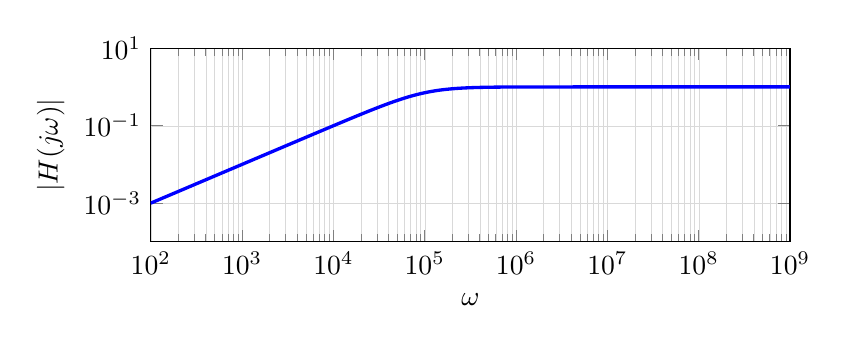
\begin{tikzpicture}[
    declare function={
    mag(\omega)= (\omega / 10^5) / sqrt(1 + (\omega / 10^5)^2)    
     %  Bode approximation
     %  mag(\omega)= (\omega < 10^5) * (\omega / 10^5) +
     %            (\omega >= 10^5) * (1)
     %
     ;
    }
  ]
    \begin{loglogaxis}[
      ymin=0.0001, ymax=10, ylabel=$|H(j \omega)|$,
      xmin=10^2, xmax=10^9, xlabel=$\omega$,
      domain=10^2:10^9,
      grid=both, grid style={line width=.1pt, draw=gray!30},
      width=\textwidth * 0.8,
      height=\textwidth / 3,
      samples=500
    ]
      \addplot [blue,very thick] {mag(x)};
    \end{loglogaxis}
    \vspace{0.3 cm}
  \end{tikzpicture}
  
  Phase (semi-log scale): The phase of $H(j \omega)$ is $\frac{\pi}{2}$ for $\omega \approx 0.$ When $\omega = \omega_{c}, \angle H(j \omega) = \frac{\pi}{4},$ for larger values of $\omega,$ it will continue to decreases until it asymptotically reaches $0$ as $\omega >> \omega_{c}.$

  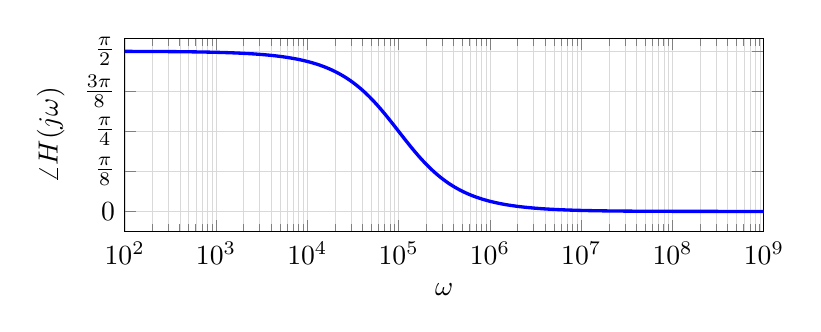
\begin{tikzpicture}[
    declare function={
    phase(\omega)= pi/2 - rad(atan(\omega / 10^5))
      % Bode approximation 
      % phase(\omega)= (\omega < 10^4) * (pi / 2) +
      %           and(\omega >= 10^4, \omega < 10^6) * (-pi / 4 * (log10(\omega) - 4) + pi / 2) +
      %           (\omega >= 10^6) * (0)
     ;
    }
  ]
  \begin{semilogxaxis}[
    ymin= -0.2, ymax=1.7, ylabel=$\angle H(j \omega)$,
    ytick={pi/2, 3*pi/8, pi/4, pi/8, 0},
    yticklabels={$\frac{\pi}{2}$,$\frac{3\pi}{8}$,$\frac{\pi}{4}$,$\frac{\pi}{8}$,$0$},
    xmin=10^2, xmax=10^9, xlabel=$\omega$,
    domain=10^2:10^9,
    grid=both, grid style={line width=.1pt, draw=gray!30},
    width=\textwidth * 0.8,
    height=\textwidth / 3,
    samples=500
  ]
    \addplot [blue,very thick] {phase(x)};
  \end{semilogxaxis}
\end{tikzpicture}
}
\end{enumerate}

\qitem What happens if we cascade these two filters together with a unity-gain buffer in between them? Consider the resulting transfer function: 
  $H(\omega) = \frac{1}{j\omega C_{1}R_{1} + 1} \cdot \frac{j\omega C_{2}R_{2}}{j\omega C_{2}R_{2} + 1}$
\begin{enumerate}
  \qitem What are the cutoff frequencies of this filter?

  \sol{
  The lower cutoff is the cutoff frequency of the high-pass filter:
  $$\omega_{c,l} = \frac{1}{R_{2}C_{2}} = 10^{5}$$
  The upper cutoff is the cutoff frequency of the low-pass filter:
  $$\omega_{c,u} = \frac{1}{R_{1}C_{1}} = 10^{8}$$
  }
  \qitem Sketch its phase and magnitude. \textit{Hint: How can we combine the plots of the individual filters together?}

  \sol{
  For both the magnitude and the phase plots, you can "add" the plots of the high-pass filter and the low-pass filter.
  This can be done since both are on a log-log scale.
  
  \begin{figure}[h]
  \textbf{Magnitude plot:}
  \centering
    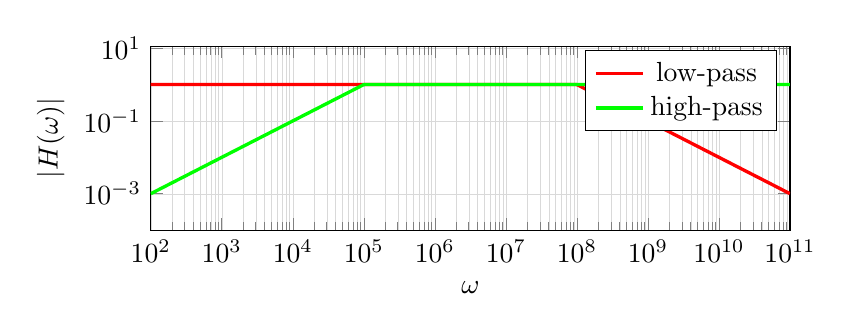
\begin{tikzpicture}[
      declare function={
        highpass(\omega)= (\omega < 10^5) * (\omega / 10^5) +
                  (\omega >= 10^5) * (1)
       ;
       lowpass(\omega)= (\omega < 10^8) * (1) +
                 (\omega >= 10^8) * (10^8 / \omega)
      ;
      }
    ]
      \begin{loglogaxis}[
        ymin=0.0001, ymax=11, ylabel=$|H(\omega)|$,
        xmin=10^2, xmax=10^11, xlabel=$\omega$,
        domain=10^2:10^11,
        grid=both, grid style={line width=.1pt, draw=gray!30},
        width=\textwidth * 0.8,
        height=\textwidth / 3.1,
        samples=500
      ]
        \addplot [red,very thick] {lowpass(x)};
        \addlegendentry{low-pass}
        \addplot [green,very thick] {highpass(x)};
        \addlegendentry{high-pass}
      \end{loglogaxis}
    \end{tikzpicture}
  \end{figure}

  \begin{figure}
  \centering
    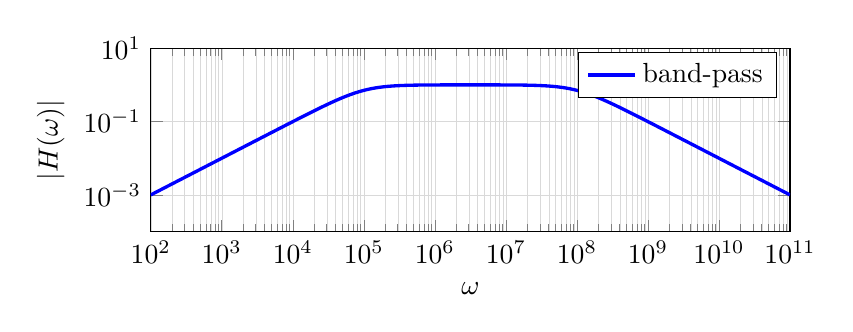
\begin{tikzpicture}[
      declare function={
      highpass(\omega)= (\omega / 10^5) / sqrt(1 + (\omega / 10^5)^2)
      % highpass(\omega)= (\omega < 10^5) * (\omega / 10^5) +
      %           (\omega >= 10^5) * (1)
      ;
      lowpass(\omega)= 1 / sqrt(1 + (\omega / 10^8)^2)
       % lowpass(\omega)= (\omega < 10^8) * (1) +
       %           (\omega >= 10^8) * (10^8 / \omega)
      ;
      }
    ]
      \begin{loglogaxis}[
        ymin=0.0001, ymax=10, ylabel=$|H(\omega)|$,
        xmin=10^2, xmax=10^11, xlabel=$\omega$,
        domain=10^2:10^11,
        grid=both, grid style={line width=.1pt, draw=gray!30},
        width=\textwidth * 0.8,
        height=\textwidth / 3.1,
        samples=600
      ]
        \addplot [blue,very thick] {lowpass(x) * highpass(x)};
        \addlegendentry{band-pass}
        
      \end{loglogaxis}
    \end{tikzpicture}
  \end{figure}

  \begin{figure}[!h]
  \textbf{Phase plot:}
  \centering

    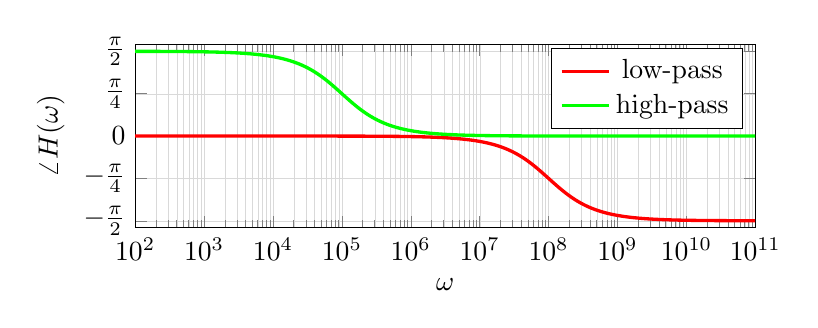
\begin{tikzpicture}[
      declare function={
      lowpass(\omega) = -rad(atan(\omega / 10^8))
        % lowpass(\omega)= (\omega < 10^7) * (0) +
        %           and(\omega >= 10^7, \omega < 10^9) * (-pi / 4 * (log10(\omega) - 7)) +
        %           (\omega >= 10^9) * (-pi / 2)
       ;
      highpass(\omega) = pi/2 - rad(atan(\omega / 10^5))
       % highpass(\omega)= (\omega < 10^4) * (pi / 2) +
       %           and(\omega >= 10^4, \omega < 10^6) * (-pi / 4 * (log10(\omega) - 4) + pi / 2) +
       %           (\omega >= 10^6) * (0)
      ;
      }
    ]

      \begin{semilogxaxis}[
        ymin= -1.7, ymax=1.7, ylabel=$\angle H(\omega)$,
        ytick={-pi/2, -pi/4, 0, pi/4, pi/2},
        yticklabels={$-\frac{\pi}{2}$,$-\frac{\pi}{4}$,$0$,$\frac{\pi}{4}$,$\frac{\pi}{2}$},
        xmin=10^2, xmax=10^11, xlabel=$\omega$,
        domain=10^2:10^11,
        grid=both, grid style={line width=.1pt, draw=gray!30},
        width=\textwidth * 0.78,
        height=\textwidth / 3.1,
        samples=500
      ]
        \addplot [red,very thick] {lowpass(x)};
        \addlegendentry{low-pass}
        \addplot [green,very thick] {highpass(x)};
        \addlegendentry{high-pass}
      \end{semilogxaxis}
  \end{tikzpicture}
\end{figure}

\begin{figure}[!h]
\centering

  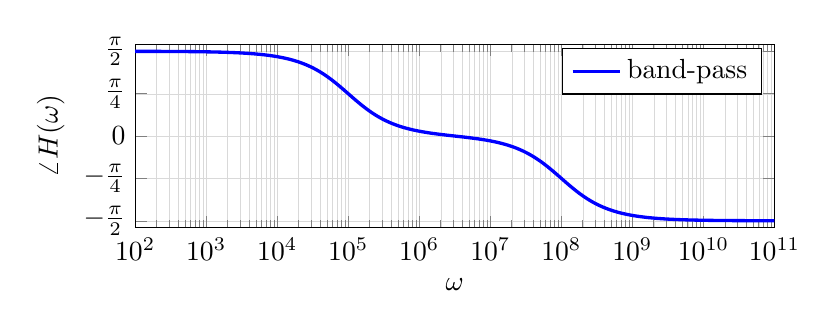
\begin{tikzpicture}[
    declare function={
    lowpass(\omega) = -rad(atan(\omega / 10^8))
      % lowpass(\omega)= (\omega < 10^7) * (0) +
      %           and(\omega >= 10^7, \omega < 10^9) * (-pi / 4 * (log10(\omega) - 7)) +
      %           (\omega >= 10^9) * (-pi / 2)
     ;
    highpass(\omega) = pi/2 - rad(atan(\omega / 10^5))
     % highpass(\omega)= (\omega < 10^4) * (pi / 2) +
     %           and(\omega >= 10^4, \omega < 10^6) * (-pi / 4 * (log10(\omega) - 4) + pi / 2) +
     %           (\omega >= 10^6) * (0)
    ;
    }
  ]

    \begin{semilogxaxis}[
      ymin= -1.7, ymax=1.7, ylabel=$\angle H(\omega)$,
      ytick={-pi/2, -pi/4, 0, pi/4, pi/2},
      yticklabels={$-\frac{\pi}{2}$,$-\frac{\pi}{4}$,$0$,$\frac{\pi}{4}$,$\frac{\pi}{2}$},
      xmin=10^2, xmax=10^11, xlabel=$\omega$,
      domain=10^2:10^11,
      grid=both, grid style={line width=.1pt, draw=gray!30},
      width=\textwidth * 0.8,
      height=\textwidth / 3.1,
      samples=500
    ]
    \addplot [blue,very thick] {lowpass(x) + highpass(x)};
    \addlegendentry{band-pass}
    \end{semilogxaxis}
  \end{tikzpicture}
  \end{figure}
  }
  \meta{
  We can "add" the magnitudes of the high-pass and low-pass filters together because we are graphing $log(|H(\omega)|) = log(|H_{high}(\omega)| \cdot |H_{low}(\omega)|) = log(|H_{high}(\omega)|) + log(|H_{low}(\omega)|)$.
  We can "add" the phases because $\angle(H_{high}(\omega) * H_{low}(\omega)) = \angle(H_{high}(\omega)) + \angle(H_{low}(\omega))$.
  }
  \end{enumerate}
\end{enumerate}
Now lets take a look at two more concepts, \textbf{bandwidth} and \textbf{Q-factor}. The bandwidth of a resonance
circuit is the difference between its upper and lower cutoff frequencies. It can also be expressed as \textit{resonance frequency} divided by its \textit{Q-factor}:

\begin{align}
    bandwidth = \Delta \omega = f_{high} - f_{low} = \frac{\omega_n}{Q}
\end{align}

The Q-factor, or quality factor, of a circuit is the ratio of power stored to power dissipated, but can also be more simply thought of as the measure of how good a circuit is,
where a higher Q-factor is often more desirable. This can be expressed mathematically as:

\begin{align}
    Q = \frac{\omega_{n}}{\Delta \omega}
\end{align}

\meta{
Circuits that have low bandwidths relative to their center frequency will have higher Q-factors.
}

\begin{enumerate}[resume]
  \qitem Find the bandwidth of this circuit.

  \sol{
  $$\Delta \omega = \omega_{c,u} - \omega_{c,l} = \frac{1}{R_{1}C_{1}} - \frac{1}{R_{2}C_{2}}$$
  $$\Delta \omega = 10^{8} - 10^{5} = 9.99 \cdot 10^{7}$$
  }
  \qitem What is its Q-factor? I.e.: $\frac{\omega_{n}}{\Delta \omega}$, where $\omega_{n}$ is the center frequency of the band.
  
  \sol{
  Symbolically:
  $$Q = \frac{\omega_{n}}{\Delta \omega} = \frac{\frac{1}{2}  \cdot (\frac{1}{R_{1}C_{1}} + \frac{1}{R_{2}C_{2}})}{\frac{1}{R_{1}C_{1}} - \frac{1}{R_{2}C_{2}}}$$
  $$Q = \frac{(R_{2}C_{2} + R_{1}C_{1})}{2 \cdot (R_{2}C_{2} - R_{1}C_{1})}$$
  Numerically:
  $$Q = \frac{\omega_{n}}{\Delta \omega} = \frac{1/2 (10^{8} + 10^{5})}{9.99 \cdot 10^{7}} = \frac{5.005 \cdot 10^{7}}{9.99 \cdot 10^{7}}$$
  $$Q \approx 0.501$$
  }
\end{enumerate}
% \end{enumerate}
